% Chapter 2 - Network perspective of open innovation 
\section{Introduction}

The previous chapter defined open innovation as \enquote{a distributed innovation process that relies on purposely managed knowledge flows across organisational boundaries, using pecuniary and non-pecuniary mechanisms in line with the organisation’s business model} \citep{chesbrough2014explicating}. Because open innovation involves multiple organisations exchanging knowledge with one another, an open innovation partnership can be conceptualised as a temporary knowledge network, one that has been set up to achieve a specific innovation outcome within a market relevant time-frame \citep{perez2013temporary,cococcioni2014exploring}. \medskip
% temporary organisation
We argue that under such conditions, the organization can benefit by forming temporary networks (TNs) and renewing, reconfiguring, creating, aligning, and directing the TN’s resources. TNs are those that are formed quickly and last a short period of time. We label the dynamic capability to form TNs and manage TNs’ resources as temporary network development capability (TNDC) and suggest that it is a special kind of relational capability \citep{perez2013temporary}.

How easily knowledge flows through a knowledge network depends on various internal (endogenous) and external (exogenous) factors. Endogenous factors refer to the self\hyp{}organising processes that give rise to specific network configurations, e.g. network closure reflects a human tendency to form social groups \citep{robins2015doing}. Exogenous factors include a diverse range of environmental, human, and organisational factors that shape the development of social relations. For instance, actors in a network may connect because they share something in common. Alternatively, new types of relations may arise from preexisting relations, e.g. longstanding suppliers may become innovation partners. Other exogenous factors such as prevailing culture, geography, language, and industry setting may also influence the development of knowledge relations. We can use social network analysis to assess knowledge exchange processes in open innovation networks and the extent to which these are shaped by endogenous and exogenous factors. A network perspective will offer fresh insights into the social processes that underpin open innovation. \medskip

This chapter has two parts: The first part introduces key concepts in social network analysis. This includes some basic network terminology and an overview of commonly used network measures. The second part explores how knowledge networks facilitate innovation and highlights some of the key challenges in inter\hyp{}organisational knowledge transfer. \medskip

\section{Basic network terminology and notation}

\subsection{Social networks}

A social network is a way to conceptualise a social system in terms of the structure of relationships among social actors. Usually, a social network is represented as a mathematical graph with vertices and edges, where vertices represent actors (also referred to as nodes) and the edges the ties (or social connections) between them (Figure \ref{fig:examples}). \medskip

\begin{figure}
	\centering
	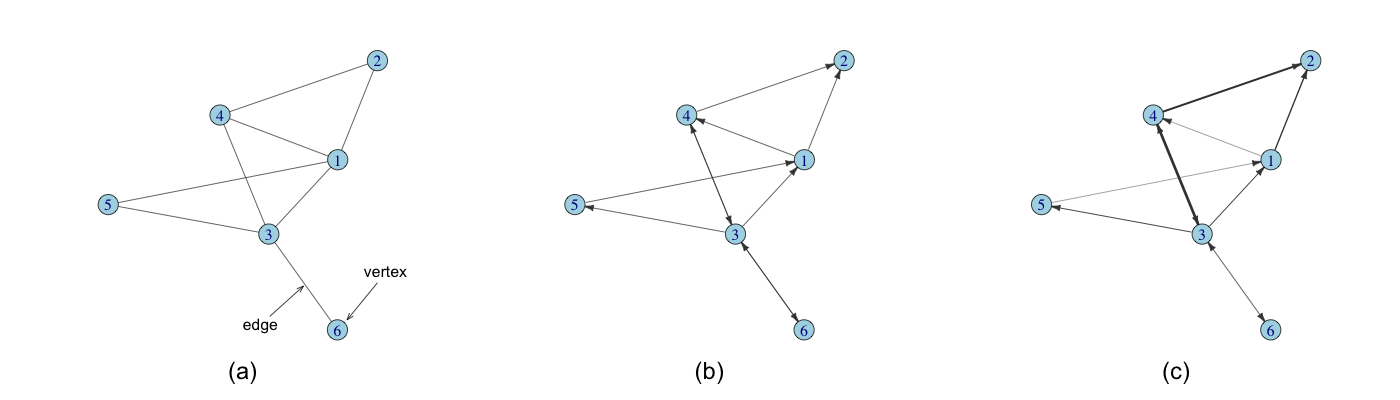
\includegraphics[width=1.0\linewidth]{Images/example_networks.png}
	\caption{Example network with (a) undirected binary ties, (b) directed binary ties, and (c) valued ties (edges are weighted according to some value).}
	\label{fig:examples}
\end{figure}

 Actors may be distinguished by binary, categorical or continuous attributes. For example, consider an individual actor classified as female (binary attribute), who works for a particular organisation (categorical attribute), with a specific number of years work experience (continuous attribute). Ties between actors can be measured as directed or undirected, and as binary or valued. Deciding whether to measure a tie as directed or undirected depends on the nature of the tie. For instance, ties indicating organisational affiliation are inherently undirected, whereas authority is essentially directed \citep{borgatti2013analyzing}. \medskip
 
 Figure \ref{fig:tie_type} characterises different types of social ties. Ties can be either continuous or discrete in nature \citep{borgatti2013analyzing}. We can describe continuous ties in terms of similarity or social relations. Ties between actors who share something in common (e.g. work at the same location, are affiliated to the same body, participate in the same event, or share a common attribute) are referred to as similarity ties. Actors can have many different kinds of social relations, e.g. friendship, knowledge sharing, advice seeking, and reporting ties. Relational ties can also be affective (like or dislike another actor) or perceptual (belief about the other actor). Discrete ties refer to ties defined by specific social interactions (e.g. a transaction of some kind, attendance at the same event) and flows (e.g. communication or knowledge flows). \medskip

Ties are often interdependent, i.e. the presence of one tie affects the presence of others. Without some form of dependence among ties, it is often difficult to explain why certain patterns of ties form \citep{lusher2013exponential}. An example is friendship, which usually develops in the presence of an preexisting similarity tie (e.g. both actors share a common interest or work at the same place) or via a interaction tie (e.g. actors were introduced to each other at a specific event or worked together on a particular project). \medskip

\begin{figure}
	\centering
	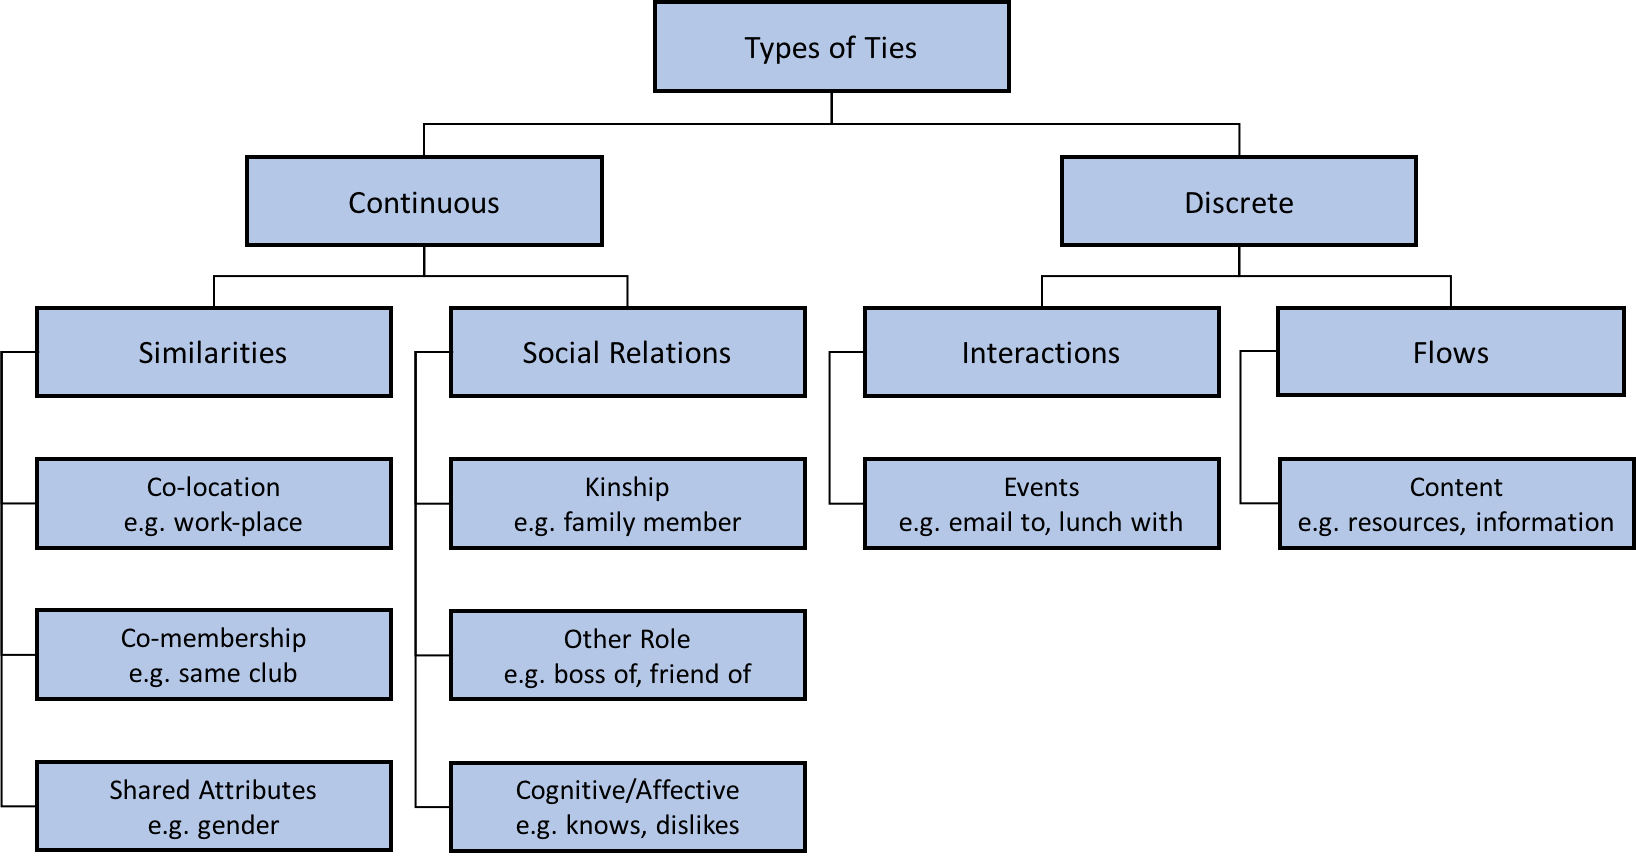
\includegraphics[width=0.9\linewidth]{tie_type}
	\caption{Different types of social ties \citep{borgatti2013analyzing}.}
	\label{fig:tie_type}
\end{figure}

\subsection{Network data structures}

A social network can be described as having a given set of $n$ actors, with variables $X_{ij}$ representing how actor $i$ is tied to actor $j$. Edge lists and adjacency matrices are the most commonly used data structures for social networks. With an edge list, an edge between two actors $i$ and $j$ is denoted as $(i,j)$, so that a complete network with $n$ actors can be specified by giving the value $n$ and a list of edges. \medskip

The edge list for the undirected binary network depicted in Figure \ref{fig:examples} would have $n = 6$ actors and edges $(1,2),(1,3),(1,4),(1,5),(2,4),(3,4),(3,5),(3,6)$. A directed network has twice the number of total possible edges than an undirected network (directed network edges can be bi\hyp{}directional). Thus, the edge list for the directed binary network depicted in Figure \ref{fig:examples} would have $n = 6$ actors and edges $(1,2),(1,4),(3,1),(3,4),(3,5),(3,6),(4,2),(4,3),(5,1),(6,3)$. \medskip

Though edge lists are an efficient way to represent networks, they are too cumbersome for computational operations \citep{newman2010networks}. An adjacency matrix is a better way to represent and manipulate social network data \citep{hummon1990computational}. For a social network $X$ the adjacency matrix would be an $n \times n$ matrix with elements $X_{ij}$. In the case of a binary network, the adjacency matrix would be expressed as follows: 
\[
X_{ij} =
\begin{cases}
    1 & \text{if  } i \rightarrow j \\
    0 & \text{otherwise}
\end{cases}
\]
For an undirected network, $X_{ij}$ and $X_{ji}$ are equal. With a directed network, $X_{ij}$ and $X_{ji}$ are treated as different variables, either with the same or different values. For a directed binary network, values = 1 in the $i$th row of an adjacency matrix represent ties sent by actor $i$, and the values = 1 in the $j$th column of an adjacency matrix represent ties received by actor $j$. The adjacency matrix representing the directed and undirected binary networks depicted in Figure \ref{fig:examples} would be expressed as: $$
X_{ij} =
\left \{
  \begin{tabular}{cccccc}
    0 & 1 & 0 & 1 & 0 & 0 \\
    0 & 0 & 0 & 0 & 0 & 0 \\
    1 & 0 & 0 & 1 & 1 & 1 \\
    0 & 1 & 1 & 0 & 0 & 0 \\
    1 & 0 & 0 & 0 & 0 & 0 \\
    0 & 0 & 1 & 0 & 0 & 0
  \end{tabular}
\right \}
$$ 
With non-binary or valued networks, the presence of a tie is indicated by some value (usually a real number, not equal to 0) that describes a property of the tie e.g. tie-strength, interaction frequency, or some measure of resource exchange. \medskip

Using adjacency matrices to represent ties among actors allows one to measure patterns of social interaction by performing a range of statistical operations based on matrix algebra \citep{anderson1999p}. \medskip

\subsection{Social network analysis}

Social network analysis is about detecting and interpreting patterns of social ties between actors \citep{de2011exploratory}. Three key assumptions about patterned relations and their effects underpin social network analysis. First, structural relations are more important than actor attributes for understanding observed behaviour. For instance, an actor may be well-qualified to perform a specific task, but is unable to do the task because the requisite relationships are not in place. Second, social networks shape and are shaped by the perceptions, beliefs, and actions of actors (the \enquote{structure versus agency} debate). Third, structural relations are dynamic, i.e. network structures are never static and are constantly evolving \citep{knoke2008social}. \medskip

Egocentric network analysis focuses on the structure of an actor's personal network (the ego's network) and what this means for that actor. Sociocentric network analysis considers patterns of social interaction between all the actors in a predefined and bounded population \citep{kilduff2003social,provan2007interorganizational}. Mixed\hyp{}method social network analysis combines quantitative and qualitative approaches in more rigorous ways to better understand the practices and conditions that produce certain network outcomes \citep{dominguez2014mixed}. \medskip

\subsubsection{Graph\hyp{}based measures}

Some of the more commonly used graph\hyp{}based measures include network density, actor centrality, and network clustering coefficients. Network density measures the overall level of connectivity in a social network. It is simply the proportion of actual (observed) ties to total number of possible ties:  $$\rho = \frac{\sum_{ij}^{n}X_{ij}}{n(n-1)}(i \neq j)$$ where $\rho$ is network density, $\sum_{ij}^{n}X_{ij}$ is the number of observed ties, and $n(n-1)$ is the total number of possible ties. Density ranges from 0 (nobody is connected) to 1 (everybody is connected to one another). The denser the network, the higher the level of cohesion and the level of redundancy in the network \citep{newman2010networks}. Knowledge is able to flow much more easily in dense networks than in sparse networks. \medskip

As the term implies, centrality measures an actor's importance in a social network \citep{borgatti2013analyzing}. There are a few ways to measure centrality, each focused on a different aspect of centrality \citep{freeman1979centrality}. Commonly used centrality measures include \enquote{degree centrality}, \enquote{betweenness centrality}, \enquote{closeness centrality}, \enquote{eigenvector centrality}, and \enquote{network constraint}. \medskip

The simplest measure is \enquote{degree centrality}, which measures an actor's overall connectivity by counting the number of ties they have with other actors. For an undirected network with \(n\) actors, degree centrality is calculated as follows: $$ d_i=\sum_{j=1}^{n}x_{ij}(i \neq j) $$ where $d_i$ is the degree centrality for actor $i$ and $\sum_{j=1}^{n}(x_{ij})$ counts the number of direct ties that $i$ has to $n-1$ other $j$ actors. Actors with high degree centrality are well-connected and in a position to exert more influence or be influenced directly \citep{borgatti2013analyzing}. Directed networks have out-degree and in-degree centrality (number of ties directed away from and towards an actor, respectively). In-degree centrality is an indicator of an actor's popularity, whereas out-degree centrality is an indicator of an actor's social activity \citep{robins2015doing}. Actors with high out-degree centrality in a knowledge network would be significant providers of knowledge. They have great influence over how knowledge is put to productive use in the network. On the contrary, actors with high in-degree centrality would be significant receivers of knowledge, i.e. they are likely to be learning the most. \medskip

Betweenness and closeness centrality consider path lengths between actors (the number of ties that must be traversed to connect any two actors). Betweenness centrality measures the extent to which an actor lies on paths between other actors: $$ b_i=\sum_{i < k}\frac{g_{jik}}{g_{jk}} $$ where $b_i$ is the betweenness centrality for actor $i$, $g_{jik}$ is the number of shortest paths connecting $j$ and $k$ through $i$, and $g_{jk}$ is the total number of shortest paths connecting $j$ and $k$ \citep{freeman1979centrality}. An actor with high betweenness usually bridges otherwise disconnected parts of the network. Their removal or departure from the network can severely disrupt network connectivity and cohesion \citep{borgatti2013analyzing}. Betweenness is an important measure of an actor's control over, or ability to broker, information exchange or resource flows within a network \citep{knoke2008social,everett2016bridging}.  Closeness centrality is the sum of the length of the shortest paths between the actor and all other actors in the network: $$c_i=\frac{1}{\sum_{j}^{n}d(i,j)}(i \neq j)$$ where $c_i$ is the closeness centrality for actor $i$ and $d(i,j)$ is the distance between actors $i$ and $j$. Closeness indicates how quickly an actor can interact with others or diffuse knowledge through the network e.g. by communicating either directly or through very few intermediaries \citep{bavelas1950communication,freeman1979centrality,knoke2008social}. \medskip

Eigenvector centrality is a measure of an actor's influence in the network \citep{bonacich1987power}. The eigenvector centrality of actor $i$ is the positive multiple of the sum of adjacent eigenvector centralities: $$e_i = \frac{1}{\lambda} \sum_{j=1}^n X_{ij}e_j$$ where $\lambda \neq 0$ is a constant. This can be expressed in matrix notation as $\lambda e = Xe$, which can be solved by the eigenvalues and eigenvectors of $X$ by virtue of the Perron\hyp{}Frobenius theorem \citep{ruhnau2000eigenvector}. An actor with high eigenvector centrality is connected to other well-connected actors in the network and thus has much greater influence \citep{borgatti2013analyzing}. They are more likely to have their knowledge or ideas gain traction than an actor with low eigenvector centrality. \medskip

Network constraint is a summary index that quantifies the extent to which an actor's access to network resources is constrained \citep{burt1992structural}. It operationalises the \enquote{strength of weak ties} concept, which argues that weak ties are more likely to provide actors access to new knowledge and opportunities \citep{granovetter1973strength}. Actors who know each other well are said to have \enquote{strong} ties with one another. They tend to form close-knit groups that are more inward looking and less receptive to external knowledge. Casual acquaintances, on the other hand, can be regarded as \enquote{weak} ties. Because acquaintances often mix in different social circles, weak ties are more likely to provide actors greater access to new knowledge and opportunities \citep{granovetter1973strength}. Network constraint is calculated as follows: $$ C_i = \sum_j c_{ij} (i \neq j) $$ where $C_i$ is the network constraint on actor $i$ and $c_{ij}$ is a measure of $i$'s dependence on $j$: $$ c_{ij} = (p_{ij} + \sum_qp_{iq}p_{qj})^2 (i \neq q \ne j) $$ and $p_{ij}$ is the proportion of $i$'s time and energy spent on $j$: $$ p_{ij} = \frac{z_{ij}}{\sum_qz_{ig}} $$ where variable $z_{ij}$ measures the strength of the tie between $i$ and $j$. Network constraint is high if the actor has few but strong ties. An actor with low network constraint has greater access to distant knowledge resources through a higher number of weak ties \citep{burt1992structural}. \medskip

\subsubsection{Network processes}

Sociologists increasingly accept that social life is shaped by a limited number of social mechanisms or processes \citep{crossley2015cases}. Social processes that are particularly relevant to this network study include reciprocity, preferential attachment, network closure, homophily, and brokerage. \medskip

Reciprocity  (\(X_{ij}X_{ji}\)) is a common feature of social networks. Both social exchange and game theory suggest dyadic relationships have a tendency to be reciprocal \citep{emerson1976social,axelrod1984evolution}. Reciprocity reflects a human tendency to return helpful (or harmful) acts in kind, e.g. \enquote{you scratch my back because I have scratched yours} \citep{nowak2005evolution}. Reciprocity contributes to more balanced and stable social relations, which in turn helps build trust and strengthen ties between actors \citep{blau1964exchange}. \medskip

New actors joining a network tend to connect with other actors who are popular and thus highly visible \citep{desollaprice976general}. This attachment bias is referred to as \enquote{preferential attachment} \citep{barabasi1999emergence}, where the probability of \(j\) forming a tie with \(i\) is dependent on the degree \(k_{i}\) (for undirected networks \(P(k_{i})=\frac{k_{i}}{\sum_{j}k_{j}}\)). Such bias implies popular actors will increase their connectivity at a higher rate than less popular actors, the so-called \enquote{rich-get-richer} phenomenon or \enquote{matthew effect} \citep{desollaprice1976general,adamic2000power,easley2010power}. Preferential attachment leads to positively skewed degree distributions, with a small number of actors with very high degree centrality and many actors with lower degree centrality. This has implications for the concentration of power in social networks \citep{emerson1962power}. \medskip 

Network closure reflects a human tendency to operate in small groups (also referred to as \enquote{cliques}). Balance theory argues unbalanced relations are stressful for humans. To reduce stress, humans strive for structural balance in social relations. This usually leads to the formation of triangular social structures through a process known as transitive closure. Triangular social structures can be thought of as archetypal small groups \citep{robins2015doing}. In the case of directed networks, transitive closure can be either cyclic or hierarchical \citep{davis1967structure}. With cyclic closure, each actor in the triad has one incoming and one outgoing tie (\(X_{ij}X_{jk}X_{ki}\)). Actors are structurally equivalent and engaged in what is referred to as \enquote{generalised exchange}. This is not the case with hierarchical closure, where one actor in the triad has two incoming ties (\(X_{ij}X_{jk}X_{ik}\)), evidence of a local hierarchy. Empirical studies indicate that cyclic closure is less prevalent in social networks, pointing to the pervasiveness of hierarchies in local group structures \citep{davis1967structure}. \medskip

Homophily is the principle that contact between similar people occurs at a higher rate than among dissimilar people \citep{mcpherson2001birds}. If preferential attachment considers popularity to be attractive, homophily might be another dimension of attractiveness \citep{wang2014homophily}. Homophily implies that the distance in social characteristics translates into network distance (the number of steps or links between two actors) i.e. the greater the similarity between actors, the shorter the network distance between them. This has implications for the information people receive, the attitudes they form, and the interactions they experience \citep{mcpherson2001birds}. Individuals are more likely to exchange knowledge with like-minded or similar others \citep{su2010understanding}. Apart from limiting access to more diverse information, homophily also promotes network closure \citep{kossinets2009origins}. Though homophily may indicate a preference to connect with similar others, the underlying motives for this are not well understood. \citet{kets2016belief} argue homophily is ultimately driven by an innate need to reduce uncertainty. Homophily emerges because players find it easier to predict the instinctive reactions of members of their own group. So while homophily may limit social reach, it does contribute to more balanced and stable social relationships \citep{scott2011sage,baccara2013homophily}. Homophily may be a contributing factor with respect to not\hyp{}invented\hyp{}here and not\hyp{}shared\hyp{}here syndromes. . \medskip

Actors who know each other well are said to have \enquote{strong} ties with one another. Casual acquaintances, on the other hand, can be regarded as \enquote{weak} ties. Strong ties usually lead to transitive closure, resulting in people becoming more inward looking and less receptive to external knowledge. Because acquaintances usually mix in different social circles, weak ties are more likely to provide actors greater access to new knowledge and opportunities \citep{granovetter1973strength}. Although weak ties enhance connectivity across the network, strong ties tend to be more effective than weak ties in facilitating learning and getting things done \citep{ahuja2000collaboration,burt2004structural,rost2011strength,phelps2012knowledge}. \medskip

Brokerage may be defined as the \enquote{behaviour by which an actor influences, manages, or facilitates interactions between other actors} \citep{obstfeld2014brokerage}. Actors that bridge otherwise disconnected parts of the network are said to occupy \enquote{structural holes} in the network \citep{burt1992structural}. They have high betweenness centrality or low network constraint, and are able to control or broker information exchange or resource flows through their network of weak ties \citep{burt1992structural,hanneman2005introduction,simpson2011network}. Such actors can exploit their favoured position either to gain some form of personal advantage (known as \textit{tertius gaudens} brokerage), or to facilitate new social relations (referred to as \textit{tertius inungens} brokerage) \citep{obstfeld2005social,obstfeld2014brokerage,quintane2016brokers}. From an open innovation perspective, \emph{tertius iungens} brokerage is quite important, especially in new partnerships, where many actors do not know their fellow collaborators in the different partner organisations. Actors in open innovation partnerships who engage in \emph{tertius gaudens} brokerage are more likely to be gatekeepers who limit the free flow of knowledge \citep{obstfeld2005social}.  \medskip 

\section{Knowledge networks}

Knowledge networks represent collections of individuals and teams who come together across organisational, spatial and disciplinary boundaries to create, share or apply a body of knowledge \citep{pugh2013designing}.  


As stated at the beginning of this chapter, we can conceptualise an open innovation partnership as a temporary knowledge exchange network set up to achieve a specific innovation outcome. The network may be treated as a dynamic capability that facilitates learning and the recombination of existing knowledge \citep{kogut1992knowledge, nahapiet1998social,rothaermel2007building,perez2013temporary,felin2016designing}. 

The network design is influenced by who is leading the initiative, which open innovation process is dominant (inbound, outbound, or coupled open innovation), whether the innovation is incremental or radical in nature, the stickiness of the knowledge involved, the time-frame in which the innovation outcome has to be achieved, and how strong the appropriability regime of each partner is. 

networks are dynamic social processes that influence knowledge creation and ultimately business direction \citep{sloane and o'reilly 2013}

% phelps


% gulati
% prusack
% dyer and singh
% nahapiet & ghosal


More explicitly, knowledge sharing refers to \enquote{the provision of task information and know-how to help others and to collaborate with others to solve problems, develop new ideas, or implement policies or procedures} \citep{wang2010knowledge}. 


\section{Conclusion}

Social network analysis allows one to use centrality measures to identify important actors in open innovation networks and to assess knowledge sharing behaviour in such networks by examining specific network configurations. The interdependence of social relations can lead to complex feedback mechanisms that make interpretation of social network processes difficult. Exponential random graph models (ERGMs) are a class of statistical model for social networks that breaks a network down into its constituent network configurations. Network configurations are assumed to represent underlying social processes or mechanisms. An ERGM allows a researcher to test hypotheses or propositions about network tie formation that relate to social theory. The following chapter (Chapter 3) reviews key social theories pertinent to this study, theories that can help explain knowledge sharing behaviour in open innovation partnerships. 